\documentclass[conference]{IEEEtran}
\IEEEoverridecommandlockouts
% The preceding line is only needed to identify funding in the first footnote. If that is unneeded, please comment it out.
% \usepackage{cite}
% Enables Portuguese Brasil
% \usepackage[portuguese]{babel}
%encoding
% Enables code listing
\usepackage{listings}
%--------------------------------------
\usepackage[T1]{fontenc}
\usepackage[utf8]{inputenc}
%--------------------------------------
%Enables the use of greek letter without a math context
\usepackage{textgreek}
%--------------------------------------
%Enables hiperlinks
\usepackage[hidelinks]{hyperref}
%--------------------------------------

\usepackage{amsmath,amssymb,amsfonts}
\usepackage{algorithmic}
\usepackage{graphicx}
\usepackage{textcomp}
\usepackage{xcolor}

\usepackage{color, colortbl}

% The code style
\usepackage{color}
\definecolor{codegreen}{rgb}{0,0.6,0}
\definecolor{codegray}{rgb}{0.5,0.5,0.5}
\definecolor{codepurple}{rgb}{0.58,0,0.82}
\definecolor{backcolour}{rgb}{0.95,0.95,0.92}

\lstdefinestyle{mystyle}{
	backgroundcolor=\color{backcolour},   
	commentstyle=\color{codegreen},
	keywordstyle=\color{magenta},
	numberstyle=\tiny\color{codegray},
	stringstyle=\color{codepurple},
	basicstyle=\footnotesize,
	breakatwhitespace=false,         
	breaklines=true,                 
	captionpos=b,                    
	keepspaces=true,                 
	numbers=left,                    
	numbersep=2pt,                  
	showspaces=false,                
	showstringspaces=false,
	showtabs=false,                  
	tabsize=2
}
\lstset{style=mystyle}
%---------------------------------------

\def\BibTeX{{\rm B\kern-.05em{\sc i\kern-.025em b}\kern-.08em
		T\kern-.1667em\lower.7ex\hbox{E}\kern-.125emX}}

\title{Uma breve revisão da Mecânica Quântica para Cientistas da Computação}

\institute{Universidade Estadual Paulista Júlio de Mesquita Filho}

\author{André Furlan - ensismoebius@gmail.com}

\logo{\includegraphics[height=1cm]{unesp.png}}
\date{\the\year}

\begin{document}
	
	\frame{\titlepage}
	
	\section{Introdução}
	
	\begin{frame}{Introdução}
		
		\par Alguns fenômenos, como o \textbf{emaranhamento} e a \textbf{superposição} presentes na mecânica quântica contribuem para uma abordagem mais eficiente em termos de velocidade na execução de alguns algoritmos. A computação quântica visa explorar e utilizar esses comportamentos.
	\end{frame}

	\section{Espaço vetorial}
	
	\begin{frame}{Espaço vetorial}
		\par Um \textbf{espaço vetorial} ($V$) sobre os números complexos $\mathbb{C}$ é uma estrutura matemática que permite a representação de seus elementos (vetores) e obedece ao seguinte conjunto de regras:
		\begin{itemize}
			\item $\alpha \in \mathbb{C}, \alpha . |V_1\rangle \in V$
			\item $\vec{0} , \vec{0} + |V_1\rangle = |V_1\rangle$ (vetor nulo)
			\item $|V_1\rangle + |V_2\rangle = |V_2\rangle + |V_1\rangle$ (comutativa)
			\item $|V_1\rangle \in V, |V_2\rangle \in V \implies |V_1\rangle + |V_2\rangle \in V$
			\item $|-V_1\rangle; |V_1\rangle + |-V_1\rangle=\vec{0}, |-V_1\rangle=-|V_1\rangle$ 
			\item $|V_1\rangle + (|V_2\rangle + |V_3\rangle) = (|V_1\rangle + |V_2\rangle) + |V_3\rangle$ (associativa)
			\item $\alpha,\beta \in \mathbb{C}; \alpha (|V_1\rangle + \beta . |V_2\rangle) = \alpha . |V_1\rangle + \alpha . \beta . |V_2\rangle $ (distributiva)
		\end{itemize}
	\end{frame}

	\begin{frame}{Base de um espaço vetorial}
		\par Sendo $V$ um espaço vetorial, sua base é o conjunto $b$ é tal que $b \subset V$ e os elementos de $b$ são ortonormais, ou seja, ortogonais entre si e unitários. \newline
		\par Em mecânica quântica esses \textbf{vetores base} são chamados de \textbf{possíveis estados do sistema}.
	\end{frame}

	\section{Notação de Dirac e os estados quânticos}

	\begin{frame}{Notação de Dirac}
		\par O estado de um sistema quântico é descrito usando um formalismo chamado \textbf{vetores de estado}, que pertencem a um \textbf{espaço vetorial} associado ao sistema. Esses vetores são geralmente denotados usando a notação "ket", introduzida pelo físico Paul Dirac, onde um vetor de estado é representado como $|\psi\rangle$, pronunciado como "ket psi".\newline
		\par A combinação dos símbolos $|$ e $\rangle$ com um valor dentro deles é chamada de "ket". Um exemplo é demonstrado na Equação \ref{eq:ketNotationVector} \cite{notacaoDirac}.
		\begin{equation}
			\ket{K} = \vec{K} = \begin{bmatrix}
				a \\
				b \\
				c \\
				d
			\end{bmatrix}
			\label{eq:ketNotationVector}
		\end{equation}
		\par Onde $a, b, c, d \in \mathbb{Q}$ e são componentes do \textbf{vetor} (ou matriz coluna) $K$.
	\end{frame}

	\begin{frame}[allowframebreaks]{Notação de Dirac para os estados quânticos}
		\par Para descrever o estado de uma partícula usando \textbf{vetores base}, o estado da partícula pode ser escrito usando a equação \ref{eq:ketNotationGeneric}.
		\begin{equation}
			\ket{\psi} = \alpha . \ket{V_1} + \beta . \ket{V_2}
			\label{eq:ketNotationGeneric}
		\end{equation}
		\par Com $\alpha$ e $\beta$ conhecidos como \textbf{amplitudes de probabilidade}.
		
		\begin{columns}
			\begin{column}{0.5\textwidth}
				\begin{figure}[h]
					\centering
					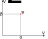
\includegraphics{../text/images/diracPlot}
					\caption{Representação visual da Equação \ref{eq:ketNotationGeneric}. $V_1$ e $V_2$ devem ser ortogonais e normalizados.}
					\label{fig:diracPlot}
				\end{figure}
			\end{column}
			\begin{column}{0.5\textwidth}
				\par A figura ao lado mostra espaço vetorial de duas dimensões com bases $V_1$ e $V_2$. Mas esse não é o caso da maioria das particulas. Um estado quântico bidimensional é apenas um caso particular conveniente para a computação.\newline
				\par Esse caso particular é chamado de \textbf{sistema de estados em dois níveis}. 
			\end{column}
		\end{columns}
		\par Sendo $N=$ o número de níveis e $a \in (\alpha, \beta, \gamma, \dots , \omega)$ \textbf{sistema de estados multinível} pode ser representada como uma soma:
		\begin{equation}
			\ket{\psi} = \sum_{i=1}^{N} a_i . \ket{V_i}= 
			\begin{bmatrix}
				a_{1} \\
				a_{2} \\
				\vdots \\
				a_{n}
			\end{bmatrix}
			\label{eq:multipleLevelStateSum}
		\end{equation}
	\end{frame}

	\section{Estados Quânticos}

	\begin{frame}{Estados Quânticos}
		\par Os estados quânticos são representações matemáticas que fornecem informações sobre as propriedades de um sistema físico, como a posição ou o momento de uma partícula.Ao contrário dos bits clássicos, que podem representar apenas 0 ou 1, os estados quânticos podem existir em uma superposição, onde eles representam simultaneamente vários estados possíveis\newline
		
		\par Os estados quânticos são descritos usando vetores de estado, que são frequentemente representados usando a notação de Dirac "ket" (por exemplo, $|\psi\rangle$).
	\end{frame}

	\begin{frame}{Exemplo físico}
		\par Um bom exemplo do que pode ser um estado quântico são as frequências de onda de um fóton. Essa partícula possui componentes elétricos e magnéticos, formando um campo eletromagnético. Podemos interpretar, por exemplo, a componente "vertical" como o estado 0 e a "horizontal" como o estado 1, conforme ilustrado na Figura abaixo.
		
		\begin{columns}
			\begin{column}{0.5\textwidth}
				\begin{figure}[H]
					\centering
					\includegraphics[width=0.6\linewidth]{../text/images/photonState01}
					\caption{Estado da partícula é definido pelos valores de amplitude de $\alpha$ e $\beta$ }
					\label{fig:photonstate01}
				\end{figure}
			\end{column}
			\begin{column}{0.5\textwidth}
				\par Perceba a semelhança com a representação visual da Equação de Dirac. \textbf{Isso não é um coincidência}. Neste caso a amplitude das ondas está diretamenta relacionada com o estado dessa partícula.
			\end{column}
		\end{columns}
		
	\end{frame}

	\section{Amplitude de probabilidade}
	
	\begin{frame}[allowframebreaks]{Amplitude de probabilidade}
		\par Como já dito anteriomente, sistema de estados em dois níveis, tem como parâmetros definidores os valores de  $\alpha$ e $\beta$. Esses são chamados de amplitude de probabilidade.\newline
		\par O uso de tais amplitudes se dá no cálculo da probabilidade de um estado colapsar em uma das bases, neste caso $\ket{0}$ ou $\ket{1}$. Como tais valores podem estar no domínio dos números complexos $\mathbb{C}$, precisamos introduzir o conceito de conjugado complexo de um número. Para um número $z = u + vi$, onde $z \in \mathbb{C}$, seu conjugado é denotado como $z^*$, onde $z^* \in \mathbb{C}$, e é dado por $z^* = u - vi$. Em resumo, se $z = u + vi$, então $z^* = u - vi$. \newline
		
		Aplicando o conceito de conjugado complexo, podemos ver que $z \cdot z^* = (u + vi) \cdot (u - vi) = u^2 + v^2 \in \mathbb{R}$. Isso resolve o problema, pois o produto $z \cdot z^*$ é um número real! \newline
		
		Finalmente, seja \(P(S_i)\) uma função que calcula a probabilidade do estado \(S_i\) ocorrer. Por exemplo, se \(|\psi\rangle = \alpha |S_0\rangle + \beta |S_1\rangle\), então \(P(S_0)\) e \(P(S_1)\) são definidos como mostrado nas equações \ref{eq:state0} e \ref{eq:state1} \cite{binney2013physics}.
		
		\begin{equation}
			\label{eq:state0}
			P(S_0) = \alpha . \alpha^* 
		\end{equation} 
		
		\begin{equation}
			\label{eq:state1}
			P(S_1) = \beta . \beta^* 
		\end{equation}
		
	\end{frame}

	\section{Princípio de Heisenberg}
	
	\begin{frame}[allowframebreaks]{Não se pode ter tudo}
		\par O princípio de Heisenberg se baseia no fato que a medição simultânea de certas grandezas nem sempre é posível: Se sabemos muito sobre a velocidade de uma partícula, pouco se sabe sobre sua posição; se é certa a presença de uma frequência em um sinal é difil saber quando a mesma ocorre, etc.
		\par O último exemplo supracitado é ilustrado na figuras abaixo:
		
		\begin{columns}
			\begin{column}{0.5\textwidth}
				\begin{figure}[h]
					\centering
					\includegraphics[width=1\linewidth]{../text/images/noisySignal}
					\caption[Multi-frequency signal]{Multi-frequency signal. Source: \cite{olama2011design}}
					\label{fig:noisysignal}
				\end{figure}
			\end{column}
			\begin{column}{0.5\textwidth}
					\begin{figure}[h]
						\centering
						\includegraphics[width=0.1\linewidth]{../text/images/windowedNoisySignal}
						\caption[Windowed signal]{Small windowed signal. Adapted from: \cite{olama2011design}}
						\label{fig:windowednoisysignal}
					\end{figure}
			\end{column}
		\end{columns}
		\par Perceba que, quando há acesso ao sinal por inteiro é fácil via uma transfomada de Fourrier, por exemplo, saber quais a frequências envolvidas no sinal, o mesmo não acontece qundo o foco é em alguma região de alta frequência.		
	\end{frame}

	\section{Qubit ou bit quântico}

	\begin{frame}[allowframebreaks]{Qubit ou bit quântico}
		\par Qubits existem em uma superposição dos estados 1 e 0 até serem medidos, momento em que seu estado colapsa para 1 ou 0 com probabilidades dadas por $|\alpha|^ 2$ e $|\beta|^2$ \cite{da2018introduccao}.
		
		\begin{equation}
			\ket{\psi} = \alpha . \ket{0} + \beta . \ket{1} = 
			\alpha . \begin{bmatrix}
				1 \\
				0
			\end{bmatrix} + \beta .	\begin{bmatrix}
				0 \\
				1
			\end{bmatrix} = 
			\begin{bmatrix}
				\alpha \\
				\beta
			\end{bmatrix}
			\label{eq:qubit}
		\end{equation}
	
		\begin{columns}
			\begin{column}{.5\linewidth}
				\begin{figure}
					\centering
					\includegraphics[width=0.5\linewidth]{../text/images/photonState02}
					\caption{Ao ser lido este qubit tem maior probabilidade de colapsar em 0.}
					\label{fig:photonstate02}
				\end{figure}
			\end{column}
			\begin{column}{.5\linewidth}
				\begin{figure}
					\centering
					\includegraphics[width=0.5\linewidth]{../text/images/photonState03}
					\caption{Ao ser lido este qubit tem maior probabilidade de colapsar em 1.}
					\label{fig:photonstate03}
				\end{figure}
			\end{column}
		\end{columns}
		
		\par Qubits têm a capacidade de armazenar e processar informações de maneira diferente dos bits clássicos devido à superposição. A sua capacidade, em termos de armazenamento de informação, é significativamente maior em comparação com os bits clássicos. No entanto, há um problema: quando os qubits são medidos, eles se transformam em bits clássicos. Portanto, atualmente, não é possível aproveitar ao máximo as propriedades quânticas para fins de armazenamento de dados. Além disso, os qubits podem armazenar dados não binários, como	 $\begin{bmatrix} \dfrac{1}{\sqrt{2}} \\\\ \dfrac{1}{\sqrt{2}} \end{bmatrix}$ or $\begin{bmatrix} \dfrac{1}{2} \\\\ \dfrac{\sqrt{3}}{2} \end{bmatrix}$.
		
		\framebreak
		
		\par A lista abaixo mostra a capacidade dos qubits em compração com os bits clássicos:
		
		\begin{itemize}
			\label{lst:qubits}
			\item 1 qubit = 2 bits
			\item 2 qubits = 4 bits
			\item 3 qubits = 8 bits (1 byte)
			\item 4 qubits = 16 bits
			\item 13 qubits = 8,192 bits (1 kilobyte)
			\item 23 qubits = 8,388,608 bits (1 megabyte)
			\item 33 qubits = 8,589,934,592 bits (1 gigabyte)
			\item 43 qubits = 8,796,093,022,208 bits (1 terabyte)
			\item n qubits = $2^n$ bits
		\end{itemize}
	\end{frame}
	
	\begin{frame}[allowframebreaks]{Portas Quânticas}
		\begin{itemize}
			\item Porta identidade: Mantém o qubit no mesmo estado.
			$I : \begin{bmatrix}
					1& 0 \\
					0& 1
				\end{bmatrix}$
			
			\item Porta Hadamard: Ela cria uma superposição de estados em um qubit. É representada pela seguinte matriz \cite{qcfcs}:
			$H = \frac{1}{\sqrt{2}}\begin{bmatrix}
				1 & 1 \\
				1 & -1 \\
			\end{bmatrix}$
			\item Porta X, ela inverte o estado de um qubit. É representada por:
			$X = \begin{bmatrix}
				0 & 1 \\
				1 & 0 \\
			\end{bmatrix}$
			\item Porta CNOT: A porta Controlled NOT opera em dois qubits, onde um atua como controle e o outro como alvo. É representada pela seguinte matriz:
			$CNOT = \begin{bmatrix}
				1 & 0 & 0 & 0 \\
				0 & 1 & 0 & 0 \\
				0 & 0 & 0 & 1 \\
				0 & 0 & 1 & 0 \\
			\end{bmatrix}$
		\end{itemize}
	
		\par Esta porta opera em \textbf{dois qubits}, onde um é o \textbf{qubit de controle} e o outro é o \textbf{target qubit}. Para representar o estado dos qubits combinados, é utilizada uma variação da notação ket, onde dois vetores são representados juntos. Isso é necessário porque os qubits não podem mais ser escritos separadamente devido ao emaranhamento que essa porta pode causar. As variações do ket são mostradas nas Equações \ref{eq:ketForTwoVectors00}, \ref{eq:ketForTwoVectors01} e \ref{eq:ketForTwoVectors02}.
	
		\begin{equation}
			\label{eq:ketForTwoVectors00}
			\ket{1}, \ket{0} \implies
			\ket{10} = \begin{bmatrix}
				0 \\
				1 \\
				1 \\
				0
			\end{bmatrix}				
		\end{equation}
		
		\begin{equation}
			\label{eq:ketForTwoVectors01}
			\ket{0}, \ket{0} \implies
			\ket{00} = \begin{bmatrix}
				1 \\
				0 \\
				1 \\
				0
			\end{bmatrix}				
		\end{equation}
		
		\begin{equation}
			\label{eq:ketForTwoVectors02}
			\ket{1}, \ket{1} \implies
			\ket{11} = \begin{bmatrix}
				0 \\
				1 \\
				0 \\
				1
			\end{bmatrix}				
		\end{equation}
		
		\par A porta CNOT opera em dois qubits, onde o primeiro qubit serve como controle e o segundo qubit como alvo. Conforme mostrado na Equação \ref{eq:cnotApplyed}, quando o qubit de controle está no estado $\ket{1}$, o qubit alvo sofre uma inversão. No entanto, quando o qubit de controle está no estado $\ket{0}$, o qubit de destino permanece inalterado \cite{nielsen2002quantum}.
		
		\begin{equation}
			\label{eq:cnotApplyed}
			\begin{aligned}
				&CNOT\ket{00} = \ket{00}, \\
				&CNOT\ket{01} = \ket{01}, \\
				&CNOT\ket{10} = \ket{11}, \\
				&CNOT\ket{11} = \ket{10}
			\end{aligned}
		\end{equation}
	\end{frame}
	
	\begin{frame}[allowframebreaks]
		\frametitle{Referências}
		\bibliography{../text/references.bib}
	\end{frame}
	
\end{document}